\section{Desarrollo}

\subsection{Transformación del grafo original}
Para resolver el problema planteamos la siguiente modificación del grafo original: cada ciudad c, antes representada por un único nodo, será ahora representada por 61 nodos distintos. Llamemos a cada uno de estos nodos $c_{i}$, con $0\leq i \leq 60$. Cada uno de estos significa ''estoy en la ciudad c con i litros de nafta en mi tanque''. \\
\indent En cuanto a las aristas, las dividiremos en dos grupos:
\begin{itemize}
\item Tipo A:  Las que van de un  $c_{i}$ a  $c_{i+1}$. Estas van a tener como peso el costo de cargar un litro de nafta en la ciudad c.
\item Tipo B: Las que van de una ciudad a otra. Estas aristas tendrán peso cero ya que al viajar no gasto dinero. Dos nodos $c_{i}$, $c'_{j}$, estarán conectados si y sólo si existe una ruta de $c$ a $c'$ con distancia $i-j$.
\end{itemize}

\indent Veamos que hallar un camino mínimo en el grafo, es equivalente a hallar una solución de nuestro problema. \\
\indent Comencemos por ver que existe una biyección entre los caminos de ambos grafos.\\ \\
\indent  \textbf{\underline{Demostración}:} Llamemos $G$ al grafo original y $G'$ al modificado. Y llamemos $s$ al vértice de salida, y $d$ al vértice de destino.\\
\indent Veamos primero que todo camino del grafo original está en el grafo modificado. \\
\indent Sea $C$ un camino de $s$ a $d$ en $G$. Construyamos un camino $C'$ en $G'$ que represente unívocamente a $C$. Supongamos que estoy en el i-ésimo vértice del camino, $v_{i}$. Ahora, si en $C$ cargamos $k_{i}$ litros de nafta en $v_{i}$ entonces vamos a tener $k_{i}$ aristas de tipo A moviéndose entre los distintos nodos que representan a $v_{i}$ en $C'$. Notemos que esta elección es única, pues estando en una ciudad con l litros, solo puedo cargar un litro de nafta, y hay una única arista que representa esta transición. Luego, cuando pasemos de $v_{i}$ a $v_{i+1}$, le vamos a agregar a $C'$ una arista de tipo B entre  $v_{i}$ y $v_{i+1}$. Esta arista también es única, ya que ir de una ciudad a otra tiene un costo fijo. Luego, si repetimos este proceso para cada $v_{i}$ en C, obtenemos el $C'$ que buscábamos. \\
\indent Ahora notemos que si tomamos un camino $C'$ en $G'$, las aristas de tipo A representan cuánta nafta cargo en un camino del grafo G, y las aristas de tipo B representan el movimiento entre ciudades. Sabiendo esto, la construcción del camino $C$ en $G$ resulta análogo. \\ %HACER GRAFO !!!!!!!!!!!!!!!!!!!!!!!!!!!
\indent Luego, si realizamos un algoritmo de caminos mínimos sobre el grafo modificado, el costo mínimo encontrado coincide con el costo mínimo del grafo original, que es la respuesta al problema que queríamos resolver.

\subsection{Dijkstra}
Utilizaremos Dijkstra para calcular distancia mínima de un nodo a todos sus vecinos. Algunas particularidades de Dijkstra son:
\begin{enumerate}
\item Dijkstra tiene como precondición que no haya ejes de peso negativo, lo cual nuestro problema garantiza.
\item Es similar al algoritmo de Prim, pero generalizado para una función $c_{\bullet}$ creciente.
\item Si tomamos la función $c_{+}$ este algoritmo resuelve el problema de camino mínimo desde un nodo a los demás.
\end{enumerate}

\indent El pseudocódigo de Dijkstra\footnote{fuente: teórica.} es el siguiente:
\begin{algorithm}[H]
\caption{Dijkstra$\bullet$}
\label{$Dijkstra$}
\begin{algorithmic}[1]
\Procedure{$Dijkstra_{\bullet}$}{grafo $G$, nodo $salida$, funcion $c_{\bullet}$}
\State $res$ $\gets$ crearVectorDeTama\~noConValor(cantNodos, indefinido)
\State $res[salida] \gets$ elementoNeutro($c_{\bullet}$)
\For{$i$=1,...,cantNodos-1}
\State $(x,y) \gets$ arista segura de G con mínimo $c_{\bullet}(xy)$  \Comment{Consideramos $x$ ya definido, $y$ no definido.}
\State $res[y] \gets c_{\bullet}(x,y)$
\EndFor
\State return $res$
\EndProcedure
\end{algorithmic}
\end{algorithm}

\indent En particular para la función $c_{+}$:
\begin{algorithm}[H]
\caption{Dijkstra+}
\label{$Dijkstra$}
\begin{algorithmic}[1]
\Procedure{$Dijkstra_{+}$}{grafo $G$, nodo $salida$}
\State $res$ $\gets$ crearVectorDeTama\~noConValor(cantNodos, indefinido)
\State $res[salida] \gets$ 0
\For{$i$=1,...,cantNodos-1}
\State $(x,y) \gets$ arista segura de G con mínimo $c_{+}(xy)$ \Comment{Consideramos $x$ ya definido, $y$ no definido.}
\State $res[y] \gets c_{+}(x,y)$						\Comment{res[$y$] = res[$x$]+peso($xy$)}
\EndFor
\State return $res$
\EndProcedure
\end{algorithmic}
\end{algorithm}

\indent Complejidad\footnote{fuente: clases teóricas.}: \\ \\
\indent Sea $n$ la cantidad de vértices, y $m$ la cantidad de aristas:
\begin{itemize}
\item Caso ralo: usar una cola de prioridad sobre heap con todas las aristas seguras. Costo $T(n + m) =  \mathcal{O}(mlgn)$
\item Caso general: usar diccionario de costo que contenga el valor de la mejor arista segura para cada $y \notin  V (T)$. Costo $T(n + m) = \mathcal{O}(m+nlgn)$.
\item Caso denso: implementar el diccionario de costos sobre un vector. Costo $T(n + m) = \mathcal{O}(n^{2}).$
\end{itemize}

\indent La implementación fue extraída de internet\footnote{fuente: https://www.geeksforgeeks.org/dijkstras-shortest-path-algorithm-greedy-algo-7/} y modificada para adaptarla a nuestras estructuras. Como fue implementado sobre vector la complejidad es $\mathcal{O}(n^{2})$. \\

\indent Notemos que Dijkstra nos devuelve el camino mínimo de un vértice hacia todos sus vecinos. Trasladado a nuestro problema, esto nos daría el costo mínimo de combustible que necesitamos para partir de una ciudad y llegar a cualquier otra. Sin embargo el problema nos pide saber esto mismo pero partiendo de cualquier ciudad. Es por esto que debemos llamar a Dijkstra una vez por nodo, es decir llamamos a Dijkstra n veces, lo cual transforma nuestra complejidad en $\mathcal{O}(n^{2})$. \\
\indent Sin embargo, nos faltan analizar unos detalles más, ya que no corremos el algoritmo sobre el grafo original, sino sobre una modificación. \\
\indent En primer lugar la cantidad de nodos del grafo aumenta. Si la cantidad de ciudades era $n$, la cantidad de nodos del grafo modificado será $61*n$. Pero como 61 es una constante, las complejidades teóricas no se modifican, sin embargo en la práctica la diferencia entre correr Dijkstra con $n$ nodos, y con $61*n$ nodos, puede ser notoria.\\
\indent Algo similar sucede con la cantidad de aristas. Dada una ruta del grafo original, como mucho se va a replicar 120 veces. Esto sucede cuando la arista tiene costo 1L, entonces voy de $a_{60}\rightarrow b_{59}$, ....$a_{1} \rightarrow b_{0}$ y viceversa. Además, se agrega una cantidad fija de 60*n aristas, las de tipo A. Sin embargo, como asumimos que el grafo es conexo, n=O(m). Luego la cantidad de aristas en el grafo modificado es $\mathcal{O}(cantidadDeRutas)$, por lo tanto esto tampoco afecta la complejidad teórica. \\
\indent Finalmente tiene sentido preguntarnos sobre qué nodo empezamos y sobre cuál terminamos, ya que antes cada nodo represtaba una única ciudad, y en el nuevo grafo, hay 61 nodos que representan la misma ciudad. La respuesta es que por cada ciudad $c$ nos interesa salir de un solo nodo, el que representa estar en la ciudad $c$ con 0 litros de nafta. Por esta razón, solo es necesario llamar a Dijkstra, $cantidadDeCiudades$ veces\footnote{Por esta razón, en main.cpp el for aumenta de a 61.}. Además en cuanto a los nodos de llegada solo nos interesa el caso de llegar con 0 litros, ya que en otro caso habríamos cargado nafta de más y sería subóptimo.

\subsection{Dijkstra con cola de prioridad}
Este algoritmo tiene el mismo pseudocódigo que la sección anterior. Es Dijkstra con una implementación particular de cola de prioridad. Por esta razón, como expusimos anteriormente, la complejidad teórica de cada llamado es $\mathcal{O}(mlgn)$. \\
\indent También como en el algoritmo, anterior lo llamamos n veces para computar los caminos mínimos de cada vértice hacia todos los demás. Luego la complejidad total es $\mathcal{O}(nmlgn)$.

\subsection{Bellman-Ford}
Al igual que Dijkstra, Bellman-Ford calcula los caminos mínimos desde un vértice a todos los otros.\\
\indent Su complejidad temporal es $\mathcal{O}(mn)$, y la espacial $\mathcal{O}(n+m)$. \\
\indent Pseudocódigo del algoritmo\footnote{fuente: teórica.}:

\begin{algorithm}[H]
\caption{Bellman-Ford}
\label{$BF$}
\begin{algorithmic}[1]
\Procedure{$Bellman-Ford$}{grafo $G$, nodo $salida$}
\State Crear un diccionario $D^{0}$ con $D^{0}[salida]$ = 0 y $D^{0}[y]$ = $\infty$, y $\neq$ v
\For{$i$=1,...,cantNodos-1}
\State Crear un diccionario $D^{i-1}[y]$ = mín\{ $D^{i}[x]$ + peso(xy) / $x \in N^{in}[y]$ \} $\forall$ $y \in V(G)$.
\EndFor
\State return $D^{n-1}$
\EndProcedure
\end{algorithmic}
\end{algorithm}

\indent Por lo mismo que en Dijkstra, hacemos cantidadDeCiudades llamados a Bellman-Ford, y la complejidad teórica es $\mathcal{O}(mn^{2})$, con n la cantidad de ciudades y m la cantidad de rutas.

\subsection{Floyd-Warshall}
Este algoritmo se diferencia de los anteriores en que en vez de calcular las distancias mínimas de un vértice hacia los otros, calcula las de todos los vértices hacia todos los otros. Por esta razón, no hay que llamarlo más de una vez.\\
\indent La complejidad de este algoritmo es $\mathcal{O}(n^3)$. Sin embargo, hay que notar que n no es la cantidadDeCiudades, sino que es 61*cantidadDeCiudades. Aunque la complejidad teórica no cambie, esto puede tener un impacto en el tiempo de ejecución en la práctica. Notemos además que en los algoritmos anteriores hacemos $cantidadDeciudades$ llamados, salteando otros 60 nodos por ciudad que no nos interesan para resolver el problema. Al llamar a Floyd-Warshall una única vez, estos $60*cantidadDeCiudades$ problemas que habíamos salteado, se resuelven.

\begin{comment}
El input de nuestro problema consiste en un grafo completo $G=(V,E)$ con pesos en las aristas $d: E \rightarrow N$, y un valor de nafta $c: V \rightarrow N$, y una capacidad de tanque $U$. Equivalentemente, si no nos es dado un grafo completo, podemos definir $d_{uv}$ como la distancia entre u y v en G. Nuestro objetivo es ir desde un comienzo s hacia un destino t de la forma mas barata posible. Para una fácil exposición nos concentramos en el caso en que comenzamos en s con el tanque vacío. Para el caso en que comenzamos con $\delta_{s}$ unidades de nafta, el mismo puede ser reducido de la siguiente manera: Agregamos un nuevos nodo $s_{0}$ tal que $d_{s_{0}s} = U - \delta_{s}$ y $c(s_{0}) = 0$. El problema de empezar en s con $\delta_{s}$ unidades de nafta y de empezar en $s_{0}$ con el tanque vacío usando una parada adicional, es equivalente.

Resolveremos el problema presentado utilizando la siguiente formulación basada en programación dinámica (PD):
\begin{equation*}
	D[u, g] = \text{Minimo costo de ir desde u hasta t, empezando con g unidades de nafta.}
\end{equation*}


\begin{lemma}
Sea $s = u_{1}, u_{2}, ... , u_{l}$ las paradas de recarga de una solución óptima utilizando como máximo $\Delta$ paradas.
La siguiente es una estrategia óptima para decidir la cantidad de gas que se va a llenar en cada parada:
en la parada $u_{l}$ cargamos nafta suficiente para alcanzar t con el tanque vacío; para $j <l$:
\begin{enumerate}
 	\item Si $c(u_{j}) < c(u_{j+1})$, entonces en $u_{j}$ llenamos el tanque.
 	\item Si $c(u_{j}) \geq c(u_{j+1})$, entonces en $u_{j}$ llenamos lo suficiente para llegar a $u_{j+1}$
\end{enumerate}
\end{lemma}

\textbf{\underline{Demostración:}} Si $c(u_{j}) < c(u_{j+1})$ y en la solución optima no llenamos en $u_{j}$ luego podemos incrementar la cantidad cargada en $u_{j}$ y decrementar la cantidad en $u_{j+1}$. Esto mejoraría el costo total de la solución, lo que contradice que habíamos asumido que teníamos una solución optima. Similarmente, si $c(u_{j}) \geq c(u_{j+1})$ luego podemos decrementar la cantidad de nafta cargada en $u_{j}$ e incrementar la cantidad cargada en $u_{j+1}$ (sin incrementar el costo total de la solución) hasta que se cumpla la condición.

Consideremos una parada de recarga $u \neq s$ en la solución óptima, y sea $w$ la parada justo antes de u.
El lema 1 implica que si $c(w) > c(u)$, alcanzamos u con un tanque vacío, de lo contrario alcanzamos u con $U - d(w, u)$ de nafta. Por lo tanto, en nuestra formulación de PD debemos seguir al menos n diferentes valores de gas para $u$. Sea $GV(u)$ el conjunto de tales valores, a saber:

\begin{equation*}
GV(u) = \lbrace U - d(w, u)| \ w \in V \ y \ c(w) < c(u) \ y \ d(w, u) \leq U\rbrace u \lbrace 0 \rbrace
\end{equation*}

Volviendo a nuestra formulación de programación dinámica:
Claramente, $D(t, 0) = 0$. Para otros vértices $u \neq t$ y $g \in GV(u)$, los valores óptimos obedecen la siguiente recurrencia:

\[
D(u,g) = min
	\begin{cases}
		D(v, 0) + (d_{uv} - g) c(u) 		& \text{si $c(v) \leq c(u) \vee v = t$ y $g \leq d_{uv}$ } \\
		D(v, U - d_{uv}) + (U - g) c(u) 	& \text{si $c(v) > c(u)$}
	\end{cases}
\]

Presentamos el siguiente ejemplo:

\begin{figure}[h]
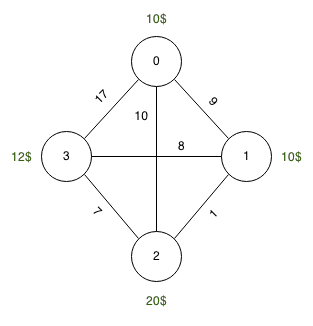
\includegraphics[width=8cm]{ex}
\centering
\end{figure}

siendo los cálculos finales:


$GV[0] = \lbrace 0 \rbrace, \ \ GV[1] = \lbrace 0 \rbrace, \ \ GV[2] = \lbrace 0, 3, 9 \rbrace, \ \ GV[3] = \lbrace 0, 2 \rbrace$


$D(0,0) = min \lbrace D(1,0) + 9 * 10 \rbrace$


$D(1,0) = min \lbrace D(2,9) + 10 * 10, D(3,0) + 8*10 \rbrace$


$D(3,0) = 0$


y asi siguiendo...

por lo tanto $D(0,0) = 170$
\end{comment}
